\documentclass[12pt,a4paper]{report}
\usepackage[utf8]{inputenc}
\usepackage{amsfonts}
\usepackage{setspace}
\usepackage{graphicx}
\usepackage{array}
\usepackage{fancyhdr}
\usepackage{geometry}
\usepackage{ragged2e}
\usepackage{color}
\usepackage{pdfpages}
\geometry{
a4paper,
total={210mm,297mm},
left=1.15in,
right=0.85in,
top=1.0in,
bottom=1.0in,
}


\begin{document}
\pagestyle{empty}
\begin{center}

{\large \textbf{Visvesvaraya Technological University, Belagavi – 590018}}
\begin{figure}[hbtp]
\centering

\includegraphics[width=2.3cm,height=2.8cm]{./pic/vtu}
\end{figure}

\textbf{PROJECT REPORT}
\par
\textbf{ON}
\par
\vspace{8pt}
{\Large\textbf{BIDIRECTIONAL COMMUNICATION SYSTEM \\[0.3em] FOR DEAF-BLIND INDIVIDUALS}}
% \parbox{\linewidth}{\centering \Large\textbf {BIDIRECTIONAL COMMUNICATION SYSTEM \\[0.1em] FOR DEAF-BLIND INDIVIDUALS}}
\par
\vspace{10pt}
\par
\textit{\textbf{Submitted in partial fulfillment for the award of degree of }}
\par
\vspace{12pt}
\large \textbf{BACHELOR OF ENGINEERING }
\par
\textbf{in}
\par
\large \textbf{COMPUTER SCIENCE \& ENGINEERING}
\par
\vspace{12pt}
\textit{\textbf{Submitted by}}
\vspace{8pt}

\textbf{\large Student Name 1}\qquad \qquad \qquad \qquad \textbf{\large 4SO20CS001}\\ \vspace{3pt} 
\textbf{\large Student Name 2}\qquad \qquad \qquad \qquad \textbf{\large 4SO20CS002}\\ \vspace{3pt}
\textbf{\large Student Name 3}\qquad \qquad \qquad \qquad \textbf{\large 4SO20CS003}\\ \vspace{3pt}
\textbf{\large Student Name 4}\qquad \qquad \qquad \qquad \textbf{\large 4SO20CS004}\\ \vspace{3pt}

\vspace{12pt}
\textit{\textbf{Under the Guidance of}}
\par
\vspace{6pt}
\textbf{Dr/Mr/Ms Guide Name }
\par
\vspace{2pt}
\normalsize { Professor/Associate/Assistant Professor, Department of CSE }
\par
\begin{figure}[hbtp]
\centering

\includegraphics[scale=0.5]{./pic/sjeclogo}
\end{figure}
\large \textbf{DEPT. OF COMPUTER SCIENCE AND ENGINEERING}
\par \Large \textbf{ST JOSEPH ENGINEERING COLLEGE}
\par 
\textbf{An Autonomous Institution}
\par
{\large{(Affiliated to VTU Belagavi, Recognized by AICTE, Accredited by NBA)}
\par
\vspace{3pt}
{\large \textbf{Vamanjoor, Mangaluru - 575028, Karnataka}}
\par 
\vspace{12pt}
{\large \textbf{2024-25}}
\end{center}
\newpage


% Certificate Page
\begin{center}
\LARGE \textbf{ST JOSEPH ENGINEERING COLLEGE}
\par
\Large \textbf{An Autonomous Institution}
\par \large{(Affiliated to VTU Belagavi, Recognized by AICTE, Accredited by NBA)}
\par \vspace{3pt}
\large \textbf{Vamanjoor, Mangaluru - 575028, Karnataka}
\par \vspace{12pt}  
\par
\large \textbf{DEPT. OF COMPUTER SCIENCE AND ENGINEERING}
\par
\begin{figure}[hbtp]
\centering

\includegraphics[scale=0.5]{./pic/sjeclogo}
\end{figure}


{\Large \textbf{CERTIFICATE}}
\end{center}
\justifying
\par
\setstretch{1.2}
\noindent 
Certified that the project work entitled \textbf{"Bidirectional Communication System for Deaf-Blind Individuals"} carried out by\vspace{0.25in} 
\par

\noindent 
\vspace{2pt} 
\textbf{\large \quad \quad \qquad Student Name 1}\qquad \qquad \qquad \qquad \textbf{\large 4SO20CS001}\\ \vspace{2pt} 
\textbf{\large \quad \quad \qquad Student Name 2}\qquad \qquad \qquad \qquad \textbf{\large 4SO20CS002}\\ \vspace{2pt}
\textbf{\large \quad \quad \qquad Student Name 3}\qquad \qquad \qquad \qquad \textbf{\large 4SO20CS003}\\ \vspace{2pt}
\textbf{\large \quad \quad \qquad Student Name 4}\qquad \qquad \qquad \qquad \textbf{\large 4SO20CS004}\\ \vspace{1pt}
\justifying

\noindent
the bonafide students of VIII semester Computer Science \& Engineering in partial fulfillment for the award of Bachelor of Engineering in Computer Science and Engineering of the Visvesvaraya Technological University, Belagavi during the year 2024-2025. It is certified that all corrections/suggestions indicated during Internal Assessment have been incorporated in the report. The project report has been approved as it satisfies the academic requirements in respect of project work prescribed for the said degree. 

\par
\vspace{0.33in}
\setstretch{1.15}
\begin{tabbing}
---------------------------------\hspace{0.3in}\=----------------------------------- \hspace{0.3in}\=--------------------------------- \\
\textbf{Dr/Mr/Ms Guide Name}\>\hspace{0.3in}\textbf{Dr Sridevi Saralaya }\>\hspace{0.3in}\textbf{Dr Rio D'Souza}\\
\hspace{0.5in}Project Guide\>\hspace{0.50in} HOD-CSE \>\hspace{0.6in}Principal
\end{tabbing}

\begin{center}
\large \textbf{External Viva}:
\end{center}
\begin{flushleft}
\begin{normalsize}Examiner's Name \end{normalsize}
\hspace{6.5cm}
\begin{normalsize}Signature with Date\end{normalsize}
\end{flushleft}
\vspace{0.1in}
\begin{flushleft}
1. \ldots\ldots\ldots\ldots\ldots\ldots \ldots \hspace{5.8cm}\ldots\ldots\ldots\ldots \ldots\ldots\ldots 
\par
\vspace{0.2in}	
2. \ldots\ldots\ldots\ldots\ldots\ldots \ldots \hspace{5.8cm}\ldots\ldots\ldots\ldots \ldots\ldots\ldots 
\end{flushleft}
\newpage

% Declaration Page
\centering
\LARGE \textbf{ST JOSEPH ENGINEERING COLLEGE}
\par
\Large \textbf{An Autonomous Institution}
\par \large{(Affiliated to VTU Belagavi, Recognized by AICTE, Accredited by NBA)}
\par \vspace{3pt}
\large \textbf{Vamanjoor, Mangaluru - 575028, Karnataka}
\par \vspace{12pt}  
\par
\large \textbf{DEPT. OF COMPUTER SCIENCE AND ENGINEERING}
\par
\begin{figure}[hbtp]
\centering

\includegraphics[scale=0.5]{./pic/sjeclogo}
\end{figure}

\begin{center}
{\Large \textbf{DECLARATION}}
\end{center}
\justifying
\par
\setstretch{1.5}
\noindent We hereby declare that the entire work embodied in this Project Report titled
\textbf{``Bidirectional Communication System for Deaf-Blind Individuals''} has been carried out by us at St Joseph Engineering College, Mangaluru under the supervision of \textbf{Dr Harivinod N,} for the award of \textbf{Bachelor of Engineering} in \textbf{Computer Science \& Engineering}. This report has not been submitted to this or any other University  for the award of any  other degree. \\
\vspace{0.25in}

\setstretch{1.5}
\begin{flushleft}
\textbf{Name of Student 1  USN:4SO20CS001}\\
\vspace{0.1in}
\textbf{Name of Student 2  USN:4SO20CS002}\\
\vspace{0.1in}
\textbf{Name of Student 3  USN:4SO20CS003}\\
\vspace{0.1in}
\textbf{Name of Student 4  USN:4SO20CS004}\\
\end{flushleft}

% \newpage
\setstretch{1.2}
\chapter*{\centering Acknowledgement}
\addcontentsline{toc}{chapter}{\numberline{}Acknowledgement}
We dedicate this page to acknowledge and thank those responsible for the shaping of the project. Without their guidance and help, the experience while constructing the dissertation would not have been so smooth and efficient.
\par
\vspace{0.15in}
\noindent We sincerely thank our Project guide \textbf{Dr Harivinod N}, Associate Professor, Computer Science and Engineering for his guidance and valuable suggestions which helped us to complete this project. We also thank our Project coordinators \textbf{Ms Supriya Salian} and \textbf{Dr Saumya Y M},  Dept of CSE, for their consistant encouragement. 
\par
\vspace{0.15in}
\noindent We owe a profound gratitude to \textbf{Dr Sridevi Saralaya}, Head of the Department, Computer Science and Engineering, whose kind support and guidance helped us to complete this work successfully
\par
\vspace{0.15in}
\noindent We are extremely thankful to our Principal, \textbf{Dr Rio D’Souza}, Director,  \textbf{Rev. Fr Wilfred Prakash D'Souza}, and Assistant Director, \textbf{Rev. Fr Kenneth Rayner Crasta} for their support and encouragement.
\par
\vspace{0.15in}
\noindent We would like to thank all faculty and staff of the Deprtment of Computer Science and Engineering who have always been with us extending their support, precious suggestions, guidance, and encouragement through the project.
\par
\vspace{0.15in}
\noindent We also extend our gratitude to our friends and family members for their continuous support.


\pagestyle{plain}
\setstretch{1.1}
\pagenumbering{roman}
\chapter*{\centering Abstract}
\addcontentsline{toc}{chapter}{\numberline{}Abstract}
% \chapter*{\centering Abstract}
% \addcontentsline{toc}{chapter}{\numberline{}Abstract}
 In a world that thrives on connectivity and communication, we often take for granted
the power of simple yet profound interactions. For individuals with sensory impairments, particularly the deaf-blind community, these fundamental human connections are often limited, making everyday life a challenge. In response to this challenge, we propose an innovative and transformative project that aims to bridge the communication gap for the deaf-blind community, enabling them to engage in text-based conversations with ease.\\

\noindent The deaf-blind community faces a profound and isolating challenge in their daily lives: the inability to access and participate in text-based communication independently. While advancements in technology have greatly improved communication for many, those who are both deaf and blind remain largely excluded from the digital world. This exclusion hinders their ability to engage in meaningful conversations, access information, and connect with others, leading to social and informational isolation \\

\noindent The project's novel solution for deaf-blind communication brings significant advantages, yielding cost savings, streamlined labor, efficient space utilization, and energy conservation. The integration of speech-to-text with real-time braille hardware interaction enhances user experience, reducing the need for extensive manual interpretation. This not only economizes resources but also fosters a more sustainable and inclusive communication solution for the deaf-blind community.

\newpage
% \linespread{0.89}
\setstretch{1.0}
% \renewcommand{\contentsname}{Table of Contents}
% \tableofcontents
% \addcontentsline{toc}{chapter}{\numberline{}Table of Contents}
\addcontentsline{toc}{chapter}{\numberline{}Table of Contents}
\renewcommand{\contentsname}{Table of Contents}
\tableofcontents
\listoffigures
\addcontentsline{toc}{chapter}{\numberline{}List of Figures}
\listoftables
\addcontentsline{toc}{chapter}{\numberline{}List of Tables}
\newpage

\pagestyle{fancy}
\fancyhf{}
\lhead{\fontsize{10}{12} \selectfont Project title}
\rhead{\fontsize{10}{12} \selectfont Chapter \thechapter}
\lfoot{\fontsize{10}{12} \selectfont Department of Computer Science and Engineering, SJEC, Mangaluru}
\rfoot{\fontsize{10}{12} \selectfont Page \thepage}
\renewcommand{\headrulewidth}{0.5pt}
\renewcommand{\footrulewidth}{0.5pt}

% \setstretch{1.0}
\linespread{0.89}
\justifying
\pagenumbering{arabic}
\chapter{Introduction}
\par
\section{Background}
In contemporary society, communication serves as the cornerstone of human interaction,
fostering connections, disseminating information, and enabling the exchange of ideas. How-
ever, for individuals confronting sensory impairments, particularly those who are both deaf
and blind, these essential channels of communication become profoundly challenging to
navigate. The deaf-blind community, often overlooked in technological advancements, faces
formidable barriers to accessing and participating in text-based communication indepen-
dently, thus exacerbating their isolation and limiting their ability to engage meaningfully
with the world.
Despite remarkable strides in technology that have revolutionized communication for
many, the unique challenges faced by the deaf-blind community persist. Traditional modes
of communication, such as sign language and tactile sign language, while invaluable, often
require face-to-face interaction or the presence of an interpreter. These limitations become
increasingly pronounced in our digital age, where accessibility to efficient and portable com-
munication solutions is paramount. As a consequence, the deaf-blind community remains
largely excluded from the benefits of the digital world, hindering their capacity to connect
with others, access information, and engage in everyday conversations.

Recognizing this significant gap in accessibility, our project proposes the development of
a Multimodal Communication System specifically tailored to the needs of individuals who
are both deaf and blind. This transformative initiative aims to empower the deaf-blind
community by providing them with a means to engage effectively in text-based conver-
sations, bridging the communication gap and enhancing their ability to connect with the
world. The project’s genesis lies in a commitment to inclusivity and the belief that technological innovation can serve as a powerful equalizer. By addressing the communication
challenges faced by the deaf-blind community, we aspire to foster a more inclusive soci-
ety where everyone, regardless of their abilities, can actively participate in the digital age.
The subsequent sections outline the scope, methodology, and feasibility considerations of
our project, providing a comprehensive roadmap for the development of the work.

\section{Problem statement }
Video digest revolves around developing algorithms and techniques to automatically create concise and coherent summaries of longer videos while retaining the essential content and context of the original footage. The primary goal is to provide an efficient representation of the video, making it easier for users to understand the video's content quickly without having to watch the entire duration. In this project we develop a query based dynamic summarization tool using deep learning techniques. 

\section{Objectives }
The aim/goal should be explained here.

Example: The aim  of the proposed project work are:
\begin{enumerate}
    \item To create a our own medicinal plant dataset
    \item To develop a deep learning algorithm with high accuracy to identify the plant
    \item To develop a web and mobile application to automatically identify the medicinal plant based on its image
\end{enumerate}

\section{Scope}
The scope of query-based video synopsis is to create a condensed and representative version of a longer video that is specifically tailored to a user's query. This allows users to quickly and efficiently find relevant information within a large video dataset.
Query-based video synopsis is important because it offers a solution to the problem of information overload in large video datasets. With the exponential growth of video data, it is becoming increasingly difficult for users to manually sift through large amounts of video content to find the information they need. Query-based video synopsis provides an automated and efficient way to extract and present the most relevant parts of the video data, making it easier for users to access and use the information they need.
Another important aspect of query-based video synopsis is its potential applications in various industries and domains. For example, in law enforcement, query-based video synopsis can help investigators quickly identify relevant video footage related to a specific crime or suspect. In education, it can be used to create condensed versions of  lecture videos for students who need to review specific topics or concepts. In marketing, it can be used to identify and extract key moments in promotional videos that are likely to be of interest to customers.
Overall, query-based video synopsis has significant scope and importance in enabling users to efficiently and effectively access relevant information from large video datasets, and it is likely to continue to play an increasingly important role in a wide range of industries and applications.

%---------------------------- Chapter TWO --------------------------

\chapter{Literature Survey}
\section{MyVox-Device for the Communication Between People: Blind, Deaf, Deaf-Blind and Unimpaired}

The paper\cite{ref1} describes the development of the MyVox device, a communication system designed for individuals who are deaf-blind. The device is powered by an ARM-based computer, specifically the Raspberry Pi, and includes a USB keyboard for input, a speaker for speech synthesis, a braille display, a vibration motor for notifications, and a real-time clock for time perception.

 The inputs of the device include a USB keyboard for text input, which can be customized to suit the user's needs, and the system also incorporates a real-time clock for time perception. The outputs of the device consist of an LCD display for text output, a speaker for speech synthesis, a braille refreshable display for tactile output, and a vibration motor for notifications. These components enable the device to provide communication capabilities for individuals who are deaf-blind, catering to their specific sensory needs and facilitating interaction with others.

The paper concludes by discussing future work, including the potential for internet access and custom applications, as well as plans to make the device available to more people in need. Overall, the MyVox device represents an important step forward in addressing the communication challenges faced by deaf-blind individuals and promoting social inclusion.

\section{Mobile Lorm Glove - Introducing a Communication Device for Deaf-Blind People }
The paper\cite{ref2} introduces the Mobile Lorm Glove, a communication device designed to support deaf-blind people's communication and enhance their independence.
The hardware prototype of the Mobile Lorm Glove includes fabric pressure sensors, vibrating motors, an ATmega328 microcontroller, shift registers, darlington transistor arrays, and a Bluetooth module for data transmission. The actuators on the glove are placed at varied distances to adjust stimulus duration, catering to individual tactile sensitivity and lorming speed. This customization allows for the adjustment of the maximal applied intensity and lorming speed to serve the user's needs.

The application scenarios for the Mobile Lorm Glove include mobile communication over distance and simultaneous translation. The glove enables the composition of text messages and their transmission to a receiver's handheld device, where the message can be read directly or translated into the Lorm alphabet using the Mobile Lorm Glove. Additionally, the glove functions as a simultaneous translator, allowing communication with individuals who are not familiar with Lorm, thus broadening the spectrum of people with whom deaf-blind individuals can engage. The device also enables parallel one-to-many communication, which can be particularly helpful in educational and learning contexts.

The Mobile Lorm Glove's input unit consists of fabric pressure sensors on the palm and a rectangular sensor on the wrist, which detect tactile input from the user's hand. These sensors transmit data to a microcontroller using a matrix design. The output unit comprises vibrating motors on the back of the glove, which provide haptic feedback based on the input received. The control unit, integrated with the microcontroller and a Bluetooth module, manages the data transmission between the glove and the user's handheld device. The user composes text messages by lorming onto their own left hand with the glove, and the data is transmitted to the handheld device for further processing or translation.

\section{Tactile Board: A Multimodal Augmentative and Alternative Communication Device for Individuals with Deafblindness}
The Tactile Board, a mobile Augmentative and Alternative Communication (AAC) device, is introduced as a groundbreaking solution to communication challenges faced by individuals with deafblindness\cite{ref3}. Characterized by dual sensory loss, deafblind individuals encounter difficulties compensating for impaired sight and hearing. The Tactile Board translates text and speech into real-time vibrotactile signs displayed through a haptic wearable, enabling deafblind individuals to communicate without direct assistance.

Based on interviews with 60 individuals with deafblindness across Europe, the Tactile Board features a 4-by-4 haptic matrix, customizable vocabulary database, and a haptic vest with coin-vibration motors. This facilitates two-way communication, addressing barriers to social interactions within the deafblind community. The paper underscores the limitations of existing technologies in meeting the unique challenges posed by dual sensory impairment, positioning the Tactile Board as a promising advancement in assistive technology.

The device's potential applications include communication with strangers, conveying environmental information, and supporting interactions in scenarios where direct touch is impractical, particularly relevant during the COVID-19 pandemic. The paper envisions future evaluations to assess the Tactile Board's impact on the confidence of individuals with deafblindness in initiating social interactions, contributing significantly to assistive technology for the deafblind community.
The Tactile Board employs a Samsung Galaxy Tab S2 tablet, Android OS, and Google's NLP API for speech recognition. RealTime Framework facilitates communication, while a Raspberry Pi and Python script translate data to on-off commands for coin-vibration motors in a haptic vest. The system incorporates 3D-printed cases and tactile tablet covers for accessibility.


\section{An Efficient Communication System for Blind, Dumb and Deaf People }
The paper\cite{ref4} outlines a project aimed at enhancing the lives of the blind, deaf, and dumb population in India, which comprises around 70 million people. The proposed system focuses on facilitating communication through sign language recognition, utilizing hand gestures for interaction between humans and computers. The system involves recording a user's voice, converting it to text on a server, classifying the text, generating corresponding signs, and transmitting them to applications for deaf or dumb individuals. Additionally, a reverse system for sign-to-speech communication is envisioned for visually impaired people. The background study references related work in object modeling, sign language character recognition, and American Sign Language translation through image processing. Technologies to be used include Blob Detection, Template Matching, and Skin Color Detection. The proposed system's characteristics include video initiation, hand sign recognition, a graphical user interface (GUI), and the ability to operate windows based on recognized signs. The system architecture involves a server for text conversion and sign generation, promoting efficient communication for the visually and hearing impaired. The conclusion emphasizes the system's potential to bridge communication gaps through image processing, enabling the recognition, storage, and use of sign language for various computer operations. 

The proposed system for enhancing communication among the blind, deaf, and dumb in India utilizes image processing techniques. Technologies include Blob Detection, Template Matching, and Skin Color Detection. The system incorporates algorithms for recognizing hand signs, translating speech to text, and generating corresponding signs for improved interaction through sign language.
\section{Multimodal Communication System for People Who Are Deaf or Have Low Vision }
The paper\cite{ref5} addresses communication challenges confronting individuals with deafness or low vision, particularly concerning standard consumer products. Profoundly deaf individuals predominantly rely on text and graphics, lacking access to verbal communication channels like radio and television. The elderly, commonly affected by visual impairment, further complicates communication, and additional disabilities can exacerbate these challenges. The research aims to develop an inexpensive real-time transformation method for verbal messages to assist the profoundly deaf and visually impaired, emphasizing the necessity for a solution with minimal visual resource requirements.

The proposed system involves transforming textual information into visual color patterns, utilizing color tagging, Morse code, and the Phonetic Alphabet for temporal coding. The design incorporates light sources, such as LEDs, with brightness modulation for improved text visualization. The limitations of Morse code for real-time communication are discussed, prompting the suggestion of a single LED coupled with glasses to enhance direct viewing. This approach aims to improve text translation and perception for the deaf and visually impaired compared to traditional codes.

In conclusion, the novel light code variant, offering enhanced dynamic perception, holds potential benefits for the deaf, visually impaired, and as a peripheral display for wearable computer applications. The proposed approach demonstrates promise in advancing communication and visual perception for diverse user groups.

\section{A Communication System for Deaf and Dumb People }
The paper\cite{ref6} addresses communication challenges for deaf and mute individuals, highlighting speech's significance. Sign language, their primary form of communication, limits interaction with the outer world. Technology, particularly hand gesture recognition within human-computer interaction (HCI), is identified as a potential solution. An "artificial speaking mouth" concept is introduced, converting captured hand gestures into speech. This innovative technique could empower mute individuals to convey thoughts naturally. The literature survey underscores the communication disadvantage faced by mute individuals compared to blind counterparts using traditional language. A proposed solution involves dumb communication interpreters, translating hand gestures into speech. Flex Sensors in a digital glove facilitate sign language translation into speech, fostering communication between mute communities and the public.

The paper introduces a real-time hand gesture recognition system for HCI, utilizing the Kinect sensor. It outlines three modules: real-time hand tracking, training gestures, and gesture recognition using hidden Markov models. Challenges in recognizing small, complex hand articulations are acknowledged, proposing Kinect for improved human-computer interaction. The proposed system aims to bridge communication gaps for speech and hearing-impaired individuals, focusing on offline recognition through four processes: Image Acquisition, Preprocessing, Feature Extraction, and Classification. Proper segmentation, feature extraction, and classification are highlighted for successful recognition, reducing data dimensionality. The procedure, implemented and tested with 26 hand gesture images, plays gesture audio files upon recognition, enabling two-way communication and enhancing speech-hearing impaired individuals' communication capabilities.

\section{On Improving GlovePi: Towards a Many-to-Many Communication Among Deaf-blind Users }
The paper \cite{ref7} introduces an enhanced version of GlovePi, a low-cost wearable device designed to facilitate communication for deaf-blind individuals. The authors emphasize the significance of assistive technologies in promoting the inclusion, integration, and independence of people with disabilities, particularly those with deaf-blindness. The proposed extension of GlovePi's architecture aims to enable many-to-many communication, addressing the need for enhanced social interaction and daily activities for deaf-blind users. By focusing on improving communication capabilities, the authors aim to enhance the overall quality of life for deaf-blind individuals. The proposed enhancements in GlovePi demonstrate a commitment to leveraging technology to address the unique communication challenges faced by individuals with deaf-blindness, ultimately contributing to their social inclusion and well-being.

\section{HaptiComm: A Touch-Mediated Communication Device for Deafblind Individuals }
The paper\cite{ref8} presents HaptiComm, a touch-mediated communication device designed to facilitate communication for Deafblind individuals. The device uses an array of electrodynamic actuators to reproduce tactile sensations of fingerspelling, allowing for communication through touch. The paper describes the design and implementation of the device, including the actuator guidance system, which was developed to cancel magnetic interference between close actuators and keep the intended skin contacts. The study evaluated the device's ability to reproduce tactile sensations of fingerspelling and the participants' ability to recognize the type and number of activated actuators. The results showed that the device was able to reproduce three of the five contact types of fingerspelling, and that participants were able to accurately recognize the type and number of activated actuators. The authors suggest that HaptiComm has the potential to improve communication for Deafblind individuals and that further investigations are needed to explore its full potential. They plan to refine the timing and speed parameters of actuation and estimate the device's individual and sequenced letter recognition rate compared to human fingerspelling. They also plan to quantify the learning curve of the device, which is an essential element in the adoption of assistive technology. 

Overall, the paper presents an innovative device that has the potential to improve communication for Deafblind individuals. The study provides valuable insights into the development and evaluation of HaptiComm, highlighting its strengths and limitations and suggesting avenues for future research.

\section{HaptiComm: A Touch-Mediated Communication Device for Deafblind Individuals }
The paper\cite{ref8} presents HaptiComm, a touch-mediated communication device designed to facilitate communication for Deafblind individuals. The device uses an array of electrodynamic actuators to reproduce tactile sensations of fingerspelling, allowing for communication through touch. The paper describes the design and implementation of the device, including the actuator guidance system, which was developed to cancel magnetic interference between close actuators and keep the intended skin contacts. The study evaluated the device's ability to reproduce tactile sensations of fingerspelling and the participants' ability to recognize the type and number of activated actuators. The results showed that the device was able to reproduce three of the five contact types of fingerspelling, and that participants were able to accurately recognize the type and number of activated actuators. The authors suggest that HaptiComm has the potential to improve communication for Deafblind individuals and that further investigations are needed to explore its full potential. They plan to refine the timing and speed parameters of actuation and estimate the device's individual and sequenced letter recognition rate compared to human fingerspelling. They also plan to quantify the learning curve of the device, which is an essential element in the adoption of assistive technology. 

Overall, the paper presents an innovative device that has the potential to improve communication for Deafblind individuals. The study provides valuable insights into the development and evaluation of HaptiComm, highlighting its strengths and limitations and suggesting avenues for future research.

\section{Proposed system}

\textbf{PLEASE NOTE: REMOVE THE QUESTION  AND WRITE ONLY THE ANSWERS \\}
\textbf{Why the Chosen Problem/Project is Important:} \\
The proposed Bidirectional Communication System for Deaf-Blind Individuals is of paramount importance as it addresses a critical and often overlooked issue, aiming to break down communication barriers and foster inclusivity. By providing a tailored solution for individuals who are both deaf and blind, the project empowers this community to actively engage in text-based communication, educational activities, and personal interactions. The system's integration in educational settings ensures equal opportunities for deaf-blind students, enabling their participation in classroom discussions and access to digital educational materials. Beyond education, the project promotes social connection by facilitating text-based communication through various channels. Moreover, it contributes to technological advancements for accessibility, reflecting a human-centric approach that recognizes and responds to the specific needs of the deaf-blind community. In essence, the project embodies the ethical responsibility of the technological community to create inclusive solutions, ultimately improving the quality of life for individuals facing unique challenges. \\



\noindent
\textbf{What is Novel in Proposed Project Work:} \\
 The proposed project distinguishes itself through a novel integration of speech-to-text conversion and braille representation, providing a multimodal communication system for deaf-blind individuals. Notably, it addresses the educational context, empowering deaf-blind students to actively engage in classroom activities and digital learning. The inclusion of real-time braille hardware interaction, an intuitive user interface designed for the unique needs of deaf-blind users, and human-centric usability testing further set this project apart. By combining these elements, the project contributes to inclusive technological innovation, emphasizing accessibility and usability to enhance the communication experience for the deaf-blind community. \\

\noindent
\textbf{How it Would Advance the State-of-the-Art:} \\
The proposed project would advance the state-of-the-art by pioneering a multimodal communication system for deaf-blind individuals, seamlessly integrating speech-to-text conversion with real-time braille hardware interaction. Its focus on educational integration and an intuitive user interface tailored to the unique needs of deaf-blind users represents a groundbreaking contribution to inclusive education and user-centered design. The project's emphasis on human-centric usability testing ensures that technological advancements align with the practical needs and preferences of the deaf-blind community, setting a new standard in assistive technology for those with combined auditory and visual impairments. Overall, the project's comprehensive approach positions it at the forefront of innovative and inclusive communication solutions, advancing the current state-of-the-art in assistive technology. \\

\noindent
\textbf{How it Differs from Existing Works:} \\
Unlike existing solutions that often focus on singular aspects of communication for the deaf-blind, the proposed project innovates through its multimodal approach, seamlessly combining speech-to-text conversion with real-time interaction with dedicated braille hardware. Its unique emphasis on educational integration, user interface tailored for the deaf-blind, and human-centric usability testing further distinguish it. The project's comprehensive communication solution, covering various facets of accessibility, sets it apart from current works, marking a pioneering advancement in assistive technology for individuals with combined auditory and visual impairments.. 
\section{Comparison of existing methods / Summary}
In Table 2.1, we've laid out a comparison of different research studies. We're taking a close look at how each study has approached its work, what methods they've used to put their ideas into action, the conclusions they've come to, and the results they've achieved. We're also noting down the challenges each study has faced.

\begin{table}[h]
    \centering
    \caption{Comparison of Existing Projects}
    \renewcommand{\arraystretch}{1.5} 
    \resizebox{\textwidth}{!}{
    \begin{tabular}{|>{\centering\arraybackslash}p{3.3cm}|>
    {\centering\arraybackslash}p{4.5cm}|>{\centering\arraybackslash}p{4.5cm}|>{\centering\arraybackslash}p{4.5cm}|>{\centering\arraybackslash}p{4.5cm}|>{\centering\arraybackslash}p{4.5cm}|}
    
        \hline
        
        \textbf{Project Title} & \textbf{Problem Addressed} & \textbf{Methodology} & \textbf{Implementation and Results} & \textbf{Inference and Results} & \textbf{Limitation/Future Scope} \\
        \hline
        Mobile Lorm Glove-Introducing a Communication Device for Deaf-Blind People (February 2012) & Communication challenges for deaf-blind individuals & Uses fabric pressure sensors, vibrating motors, and a Bluetooth module for communication & Enables mobile communication, simultaneous translation, and one-to-many communication & Enhances independence and communication for deaf-blind individuals & Thickness of the glove \\
        \hline
        Tactile Board: A Multimodal Augmentative and Alternative Communication Device for Individuals with Deafblindness (November 2020) & Communication challenges for individuals with deafblindness using a mobile AAC device & Utilizes a 4-by-4 haptic matrix, customizable vocabulary database, and a haptic vest & Employs Samsung Galaxy Tab S2, Android OS, Google's NLP API, Raspberry Pi, and Python script & Potential applications include communication with strangers and conveying environmental information. & Future evaluations are envisioned, especially during the COVID-19 pandemic \\
        \hline
        Multimodal Communication System for People Who Are Deaf or Have Low Vision (January 2002)  & Communication challenges for individuals with deafness or low vision & Involves real-time transformation of verbal messages into visual color patterns & Uses LEDs with brightness modulation for improved text visualization.& Shows promise for real-time communication for individuals with hearing and vision impairments & Acknowledges limitations of Morse code and proposes a novel light code variant. 
        \\
        \hline
        On Improving GlovePi: Towards a Many-to-Many Communication Among Deaf-blind Users (January 2018) & Communication challenges for deaf-blind individuals, emphasizing many-to-many communication & Enhanced version of GlovePi with sensors, Raspberry Pi, mobile devices, and a tuple center & Focuses on improving communication capabilities for enhanced social interaction & Aims to contribute to the social inclusion and well-being of deaf-blind individuals & Future work involves integrating output sensors for tactile feedback. \\
        \hline
        MyVox-Device for the Communication Between People: Blind, Deaf, Deaf-Blind and Unimpaired (October 2014)& Developed for individuals who are deaf-blind, addressing their communication challenges & Powered by Raspberry Pi, includes USB keyboard, speaker, braille display, vibration motor, and real-time clock & Provides customized inputs and outputs for text, speech, and tactile communication & Represents an important step in addressing the communication challenges faced by deaf-blind individuals & Future work involves internet access, custom applications, and broader availability \\
        \hline
        HaptiComm: A Touch-Mediated Communication Device for Deafblind Individuals (April 2023)&  Communication challenges for Deafblind individuals through touch-mediated communication using electrodynamic actuators & Utilizes an array of electrodynamic actuators to reproduce tactile sensations of fingerspelling, with a focus on canceling magnetic interference and addressing shaking and vibrations & Successfully reproduces three of the five contact types of fingerspelling, participants accurately recognize the type and number of activated actuators & Further investigations are needed to explore its full potential, including refining timing and speed parameters and estimating letter recognition rates compared to human fingerspelling & Acknowledges susceptibility to shaking and vibrations, plans to refine actuation parameters, estimate letter recognition rates, and quantify the learning curve \\
        \hline
    \end{tabular}
    }
    \label{tab:gesture-recognition-projects}
\end{table}



\par

%---------------------------- Chapter THREE --------------------------

\chapter{Software Requirements Specification}
\section{Functional requirements}
 \textbf{Speech-to-Text Conversion:}\\
  Integrate robust speech recognition tools or APIs, such as Google Cloud Speech-to-Text or Python's SpeechRecognition library. Capture and transcribe spoken words into written text. Ensure high accuracy in speech-to-text conversion to facilitate precise communication. 

 \noindent\textbf{Text-to-Braille Conversion:}\\
  Develop a sophisticated algorithm capable of translating transcribed text into Braille characters. Support different Braille standards and languages. Efficiency to minimize processing time for text-to-Braille conversion.

 \noindent\textbf{Braille Hardware Integration:}\\
  Integrate with Braille hardware systems i.e. device containing the sensor and actuators. Enable real-time sensory updates for seamless interaction.

 \noindent\textbf{User Interface Development:}\\
  Design an intuitive user interface for easy interaction.
  Facilitate smooth communication between the application and Braille hardware.

 \noindent\textbf{Hardware Interaction:}\\
  Develop a system that interfaces seamlessly with the chosen Braille hardware.
  Ensure the application can send Braille characters to the hardware for physical representation.
  
\section{Non-Functional requirements}
\textbf{Security Measures:}\\
Implement robust security protocols to ensure user data privacy and secure communication.

\noindent\textbf{Usability Testing:}\\
Conduct extensive usability testing with deaf-blind users to evaluate system functionality. Gather feedback for continual improvement.

\noindent\textbf{Accessibility Standards Compliance:}\\
Ensure compliance with accessibility standards to cater to the specific needs of the deaf-blind community. Test and enhance the application's compatibility with different screen reader software.

\noindent\textbf{Language and Braille Standards Support:}\\
Support Braille standards to enhance versatility and stay updated with the latest Braille standards and ensure compatibility

\section{User Interface Designs}
\textbf{Intuitive Design:}\\
\qquad Simple Navigation:
Design a straightforward navigation system that is easy for deaf-blind users to comprehend. Utilize clear and concise menu structures to facilitate intuitive interaction.

\noindent\textbf{Accessibility Features:}\\
Tactile Feedback Options:
Integrate tactile feedback options within the user interface to enhance the user experience for deaf-blind individuals. Provide customizable settings for feedback intensity and type.

\noindent\textbf{Design specifications:}\\
Maintain a consistent design language across the website and application to provide a unified user experience. Design the website to be responsive across different devices, ensuring accessibility on desktops, tablets, and smartphones.


\section{Hardware and Software requirements}
\subsection{Hardware Requirements:}

\textbf{Sensors for Braille Input:}\\
Deploy sensors capable of detecting Braille characters either through touch or proximity sensors. Ensure the sensors are responsive to user input for a seamless interaction experience.

\noindent\textbf{Actuators for Tactile Feedback:}\\
Integrate actuators to provide tactile feedback corresponding to the Braille characters displayed. Design the actuators to deliver precise and distinguishable tactile sensations for each Braille character.

\noindent\textbf{Braille Symbol Actuator/Sensor:}\\
Employ a hardware system as the primary hardware interface. Ensure the device can dynamically represent different Braille characters based on user inputs and can sense.

\subsection{Software Requirements:}

\textbf{Speech-to-Text Conversion Software:}\\
Utilize reliable speech recognition tools such as APIs, PyAudio, SpeechRecognition, and librosa by Python library for accurate conversion of spoken words into written text. Select a technology stack that supports real-time speech-to-text conversion.

\noindent\textbf{Text-to-Braille Conversion Algorithm:}\\
Develop a robust algorithm for translating the transcribed text into Braille characters using Python. Ensure the algorithm supports various Braille standards and languages.

\noindent\textbf{Braille to Hardware Translation Software:}\\
Implement software to translate the Braille characters into signals that can be understood by the hardware. Developing a communication protocol using a hardware device that can be used by sensing for seamless interaction between the software and hardware components.

\noindent\textbf{Website or Application:}\\
Create a user-friendly website or application interface for text-based communication. Include features for speech-to-text conversion, text-to-Braille conversion, and seamless interaction with the hardware.

\noindent\textbf{Operating System Compatibility:}\\
Ensure compatibility with major operating systems, such as Android and iOS, for mobile applications. For websites, ensure compatibility across different web browsers.

\noindent\textbf{Integration with ROS (Robot Operating System):}\\
Implement the necessary software components to integrate with ROS. Ensure smooth communication between different software modules.


\section{Performance Requirements }
\textbf{Real-time Speech-to-Text Conversion:}\\
Achieve near-instantaneous speech-to-text conversion. Evaluate system response time for spoken words to text. Ensure real-time transcription for effective communication.

\noindent\textbf{Efficient Text-to-Braille Translation:}\\
Swift translation of text to Braille characters. Assess the speed of the text-to-Braille conversion algorithm. Minimize delays in Braille representation.

\noindent\textbf{Seamless Hardware Interaction:}\\
Establish real-time communication with Braille hardware. Monitor time for Braille characters to be transmitted and displayed. Achieve responsive updates on the Braille hardware.

\noindent\textbf{Scalability:}\\
Ensure optimal performance with increased user interactions. Evaluate system performance under varying loads. Maintain optimal performance with a growing user base and data load.

\noindent\textbf{Resource Utilization:}\\
Optimize resource usage for efficient operation. Assess CPU, memory, and network utilization. Ensure resource-efficient operation on diverse devices.

\noindent\textbf{Error Handling:}\\
Implement effective error-handling mechanisms. Evaluate the system's ability to manage errors. Gracefully handle errors to minimize disruption.

\noindent\textbf{Usability Testing:}\\
Conduct usability testing based on user feedback. Gather feedback on system responsiveness and ease of use. Regular testing and iterative improvements for user satisfaction. 


\section{Design Constraints}
\textbf{Portability:}\\
The system must be designed for portability, considering use across different devices. Optimize the user interface and functionalities for seamless operation on various platforms, including mobile devices and desktop computers.

\noindent\textbf{Device Compatibility:}\\
Ensure compatibility with a variety of devices commonly used by the deaf-blind community. Design the system to adapt to different screen sizes, resolutions, and hardware configurations for widespread accessibility.

\noindent\textbf{Real-time Communication:}\\
Address the need for real-time communication between the application and hardware. Optimize data transmission and processing to minimize latency, providing users with immediate updates on the Braille hardware.

\noindent\textbf{Usability for Deaf-Blind Users:}\\
Prioritize usability for individuals with dual sensory impairments. Conduct usability testing with the deaf-blind community, incorporating their feedback to optimize the system's accessibility and ease of use. 

\section{Other Requirements}
\textbf{Long-term Support Plans:}\\
Develop strategies for long-term system support and updates. Establish a framework for ongoing maintenance, addressing evolving technological standards and user needs.

\noindent\textbf{Training Programs:}\\
Provide comprehensive training programs for users, educators, and support staff. Design training materials and sessions to ensure effective usage and support, promoting accessibility and user empowerment.


\chapter{System Design}
paragraph contents... 
\section{Architecture Design}
\begin{figure}[hbtp]
\centering

\includegraphics[width=4in,height=3in]{./pic/sjeclogo.png}
\label{fig:pic1}
\caption{System Architecture Diagram}
\end{figure}
This Figure \ref{fig:pic1} illustrates a high-level overview of the audio visual speech separation system. It is important to note that the specific techniques, algorithms, and models used in each component can vary depending on the implementation approach and the requirements of the system.
\section{Decomposition Description}
\begin{figure}[hbtp]
\centering

\includegraphics[width=5in,height=3in]{./pic/sjeclogo.png}
\caption{Flow chart}
\label{fig:pic2}
\end{figure}
\newpage
Figure \ref{fig:pic2} represent the flow chart of the proposed system. In audio visual speech separation, the goal is to decompose an audio signal containing multiple overlapping speakers into individual speech signals corresponding to each speaker. The decomposition process involves separating the desired speech signals from the background noise and other interfering sounds.

\section{Data Flow Design}
\par
The audio input undergoes pre-processing, while the visual input is processed to extract relevant cues. The pre-processed audio and processed visual data are then integrated. From the integrated representation, features are extracted. These features are utilized in the speech separation stage, where individual speech signals are separated from the mixture. Post-processing techniques are applied to enhance the quality of the separated speech signals. Finally, the individual speech signals are outputted as the result of the system. The data flow design ensures a sequential flow of operations, starting from capturing and processing the inputs, integrating the audio-visual information, extracting features, performing speech separation, applying post-processing, and generating the output. This design allows for effective processing and separation of audio visual data to obtain distinct speech signals from overlapping speakers.
\\
\begin{figure}[hbtp]
\centering
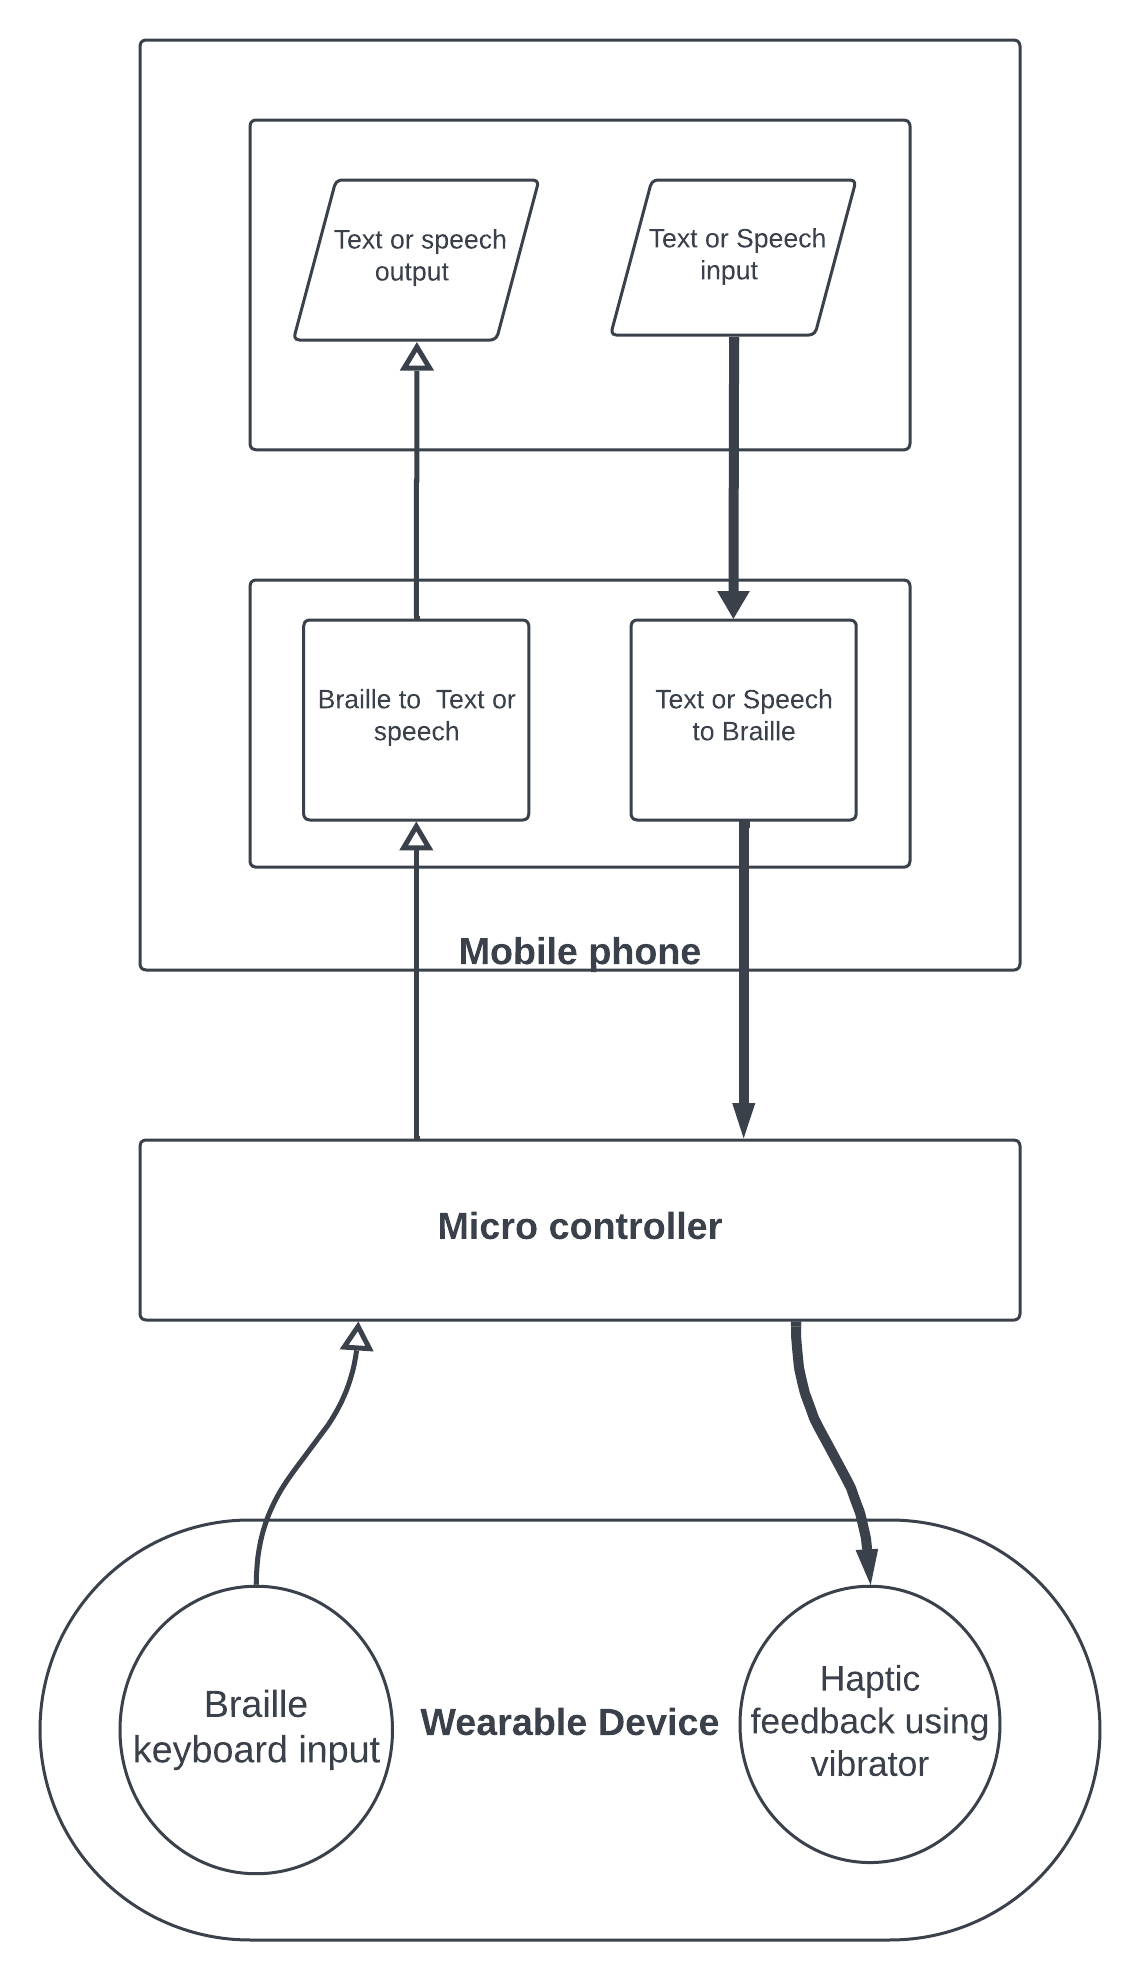
\includegraphics[width=4in,height=2in]{../fig/dataflow}
\caption{Dataflow design}
\end{figure}



\newpage
\section{Use case Diagram}
use cases represent the main functionalities and tasks involved in the audio visual speech separation system. Each use case contributes to the overall process of capturing, processing, integrating, separating, and post-processing the audio and visual data to achieve the desired outcome of individual speech signal separation.
\begin{description}
    \item [Pre-process Audio:] This use case involves pre-processing the captured audio data. It may include operations like filtering, noise reduction, and echo cancellation to improve the quality of the audio signals.

\item [Process Visual:] This use case involves processing the captured visual data. It includes tasks such as face detection, facial landmark tracking, or lip motion analysis to extract relevant visual cues associated with speech production.

\item [Integrate Audio-Visual:] This use case represents the integration of the pre-processed audio data and processed visual data to create a synchronized audio-visual representation, aligning the audio and visual streams.

\item [Extract Features:] This use case involves extracting relevant features from the integrated audio-visual representation. It may include computing spectrograms, MFCCs, facial landmarks, or other visual and audio features.

\item [Perform Speech Separation:] This use case focuses on the actual speech separation process. It utilizes the extracted audio and visual features to separate the individual speech signals from the mixture, using techniques such as blind source separation or deep learning-based models.

\end{description}

\begin{figure}[hbtp]
\centering
\includegraphics[width=9in,height=5in]{../fig/usecasess}
\caption{Use case diagram for customer}
\end{figure}


\chapter{Implementation}


\section{Audio Extraction}
\par
Audio extraction is the process of isolating and extracting the audio content from a multimedia source, such as a video file. It involves separating the audio track from the accompanying video or other elements to obtain a standalone audio file representing the sound present in the source material.

\begin{figure}[hbtp]
\centering

\includegraphics[width=5in,height=3in]{./pic/sjeclogo.png}
\caption{code snippet for audio extraction}
\end{figure}

\section{Speech Separation}
\par SpeechBrain is an open-source framework 

\subsection{Sepformer}
\par SepFormer is an algorithm for speech separation that utilizes self-attention mechanisms. It employs a transformer-based architecture to capture long-range dependencies and model the relationships between time-frequency points in the audio mixture, enabling the separation of multiple speech sources from the mixture.


\begin{figure}[hbtp]
\centering

\includegraphics[width=5in,height=3in]{./pic/sjeclogo.png}
\caption{code snippet for speech separation}
\end{figure}

\section{Speech Enhancement}
\subsection{Lite Audio Visual Speech Enhancement}
\par
Lite AVSE algorithm is used for the separation and enhancement of the speech. The system 
includes two visual data compression techniques and removes the visual feature extraction 
network from the training model, yielding better online computation efficiency. As for the audio 
features, short-time Fourier transform (STFT) is calculated of 3-second audio segments. Each 
time-frequency (TF) bin contains the real and imaginary parts of a complex number, both of 
which used as input. Power-law compression used to prevent loud audio from overwhelming soft 
audio. The same processing is applied to both the noisy signal and the clean reference signal.

\begin{figure}[hbtp]
\centering
\includegraphics[width=5in,height=3in]{../fig/codelavse}
\caption{code snippet for speech enhancement using LAVSE}
\end{figure}

\subsection{Spectral Subtraction}
Spectral subtraction is a technique used in audio signal processing to reduce background noise from an audio signal. It involves estimating the noise spectrum from a noisy signal and subtracting it from the noisy spectrum to enhance the desired signal. The resulting spectrum is then transformed back into the time domain to obtain a cleaner audio signal as in Figure \ref{fig:pic3}
\newpage
\begin{figure}[hbtp]
\centering

\includegraphics[width=5in,height=3in]{pic/sjeclogo.png}
\caption{code snippet for speech enhancement using spectral subtraction}
\label{fig:pic3}
\end{figure}

\section{Speaker Detection}
\par The cv2 functions provide methods to load the pre-trained models, apply them to images or video frames, and draw bounding boxes around the detected faces. By leveraging cv2's face detection capabilities, you can automate tasks such as facial recognition, emotion analysis, or face tracking in various applications like surveillance, biometrics, or augmented reality.


\begin{figure}[hbtp]
\centering
\includegraphics[width=5in,height=3in]{../fig/facedetect}
\caption{code snippet for speaker detection}
\end{figure}





\chapter{System Testing}
\par
Testing is a procedure of executing the program with unequivocal intension of \cite{ref4}
discovering mistakes, assuming any, which makes the program, fall flat. This stage is an
essential piece of improvement.
\par
It plays out an exceptionally basic part for quality affirmation and for guaranteeing
unwavering quality of programming. It is the way toward finding the mistakes and
missing operation and furthermore an entire confirmation to decide if the targets are met
the client prerequisites are fulfilled.
\par
The objective of testing is to reveal prerequisites, outline or coding blunders in the
projects. Therefore, unique levels of testing are utilized in programming frameworks. The
testing results are utilized amid upkeep. The testcases are shown in Figure \ref{fig:pic4}

\section{Testing Objectives}
This area manages the points of interest in the various classes of the test which should be
directed to approve capacities, imperatives and execution. This can be accomplished
fundamentally by using the methods for testing, which assumes a crucial part in the
improvement of a product.

\section{Types of Testing conducted}
The structure of the program is not being considered in useful testing. Test cases are
exclusively chosen on the premise of the prerequisites or particulars of a program or
module of program but the internals of the module or the program are not considered for
determination of experiments\cite{ref1}.

\begin{figure}[h!]
\centering

\includegraphics[width=4in,height=1in]{pic/sjeclogo.png}
\caption{testcases}
\label{fig:pic4}
\end{figure}
The program to be tried is executed with an arrangement of experiments and the yield of
the program for the experiments is assessed to decide whether the program is executing
not surprisingly. The accomplishment of testing in uncovering mistakes in projects
depends basically on the experiments. There are two fundamental ways to deal with
testing Black Box or functional Testing and White Box or structural testing. Table \ref{tab:t1} shows the workflow. 
\begin{table} [htb]
\caption {Work Flow}
\vspace{0.25in}
\begin{tabular}{|c|c|c|}\hline
\textbf{Sl No}& \textbf{Work} & \textbf{Duration(in Weeks)}\\[6pt] \hline \normalsize
1&Audio Extraction&1 \\ \hline
2&Audio Enhancement using LAVSE&4\\ \hline
3&Audio Separation using Speechbrain&3\\ \hline
4&Noice Reduction using spectral subtraction&2\\ \hline
5&Image segmentation&3\\ \hline
6&Speaker Identification&5\\ \hline
\end{tabular}
\label{tab:t1}
\end{table}



\chapter{Results and Discussion}
\section{Face detection}
\begin{figure} [hbtp]
\centering

\includegraphics[width=5in,height=4in]{pic/sjeclogo.png}
\caption{Face detection}
\label{fig:pic5}
\end{figure}
\par Above Figure \ref{fig:pic5} shows initial face detection process using opencv and dlib. It convert the image to grayscale, apply the model using cv2. detectMultiScale(), and draw bounding boxes around the detected faces using cv2.rectangle(). Display or save the result using cv2.imshow() or cv2.imwrite().

\section{Speaker recognition}
\begin{figure} [hbtp]
\centering
\includegraphics[width=5in,height=3in]{../fig/op1}
\caption{Speaker recognition 1,person 1}
\end{figure}

\begin{figure} [hbtp]
\centering
\includegraphics[width=5in,height=3in]{../fig/op2}
\caption{Speaker recognition 1,person 2}
\end{figure}

\begin{figure} [hbtp]
\centering
\includegraphics[width=5in,height=3in]{../fig/op3}
\caption{Speaker recognition 2,person 1}
\end{figure}

\begin{figure} [hbtp]
\centering
\includegraphics[width=5in,height=3in]{../fig/op4}
\caption{Speaker recognition 2,person 2}
\end{figure}

\begin{figure} [hbtp]
\centering
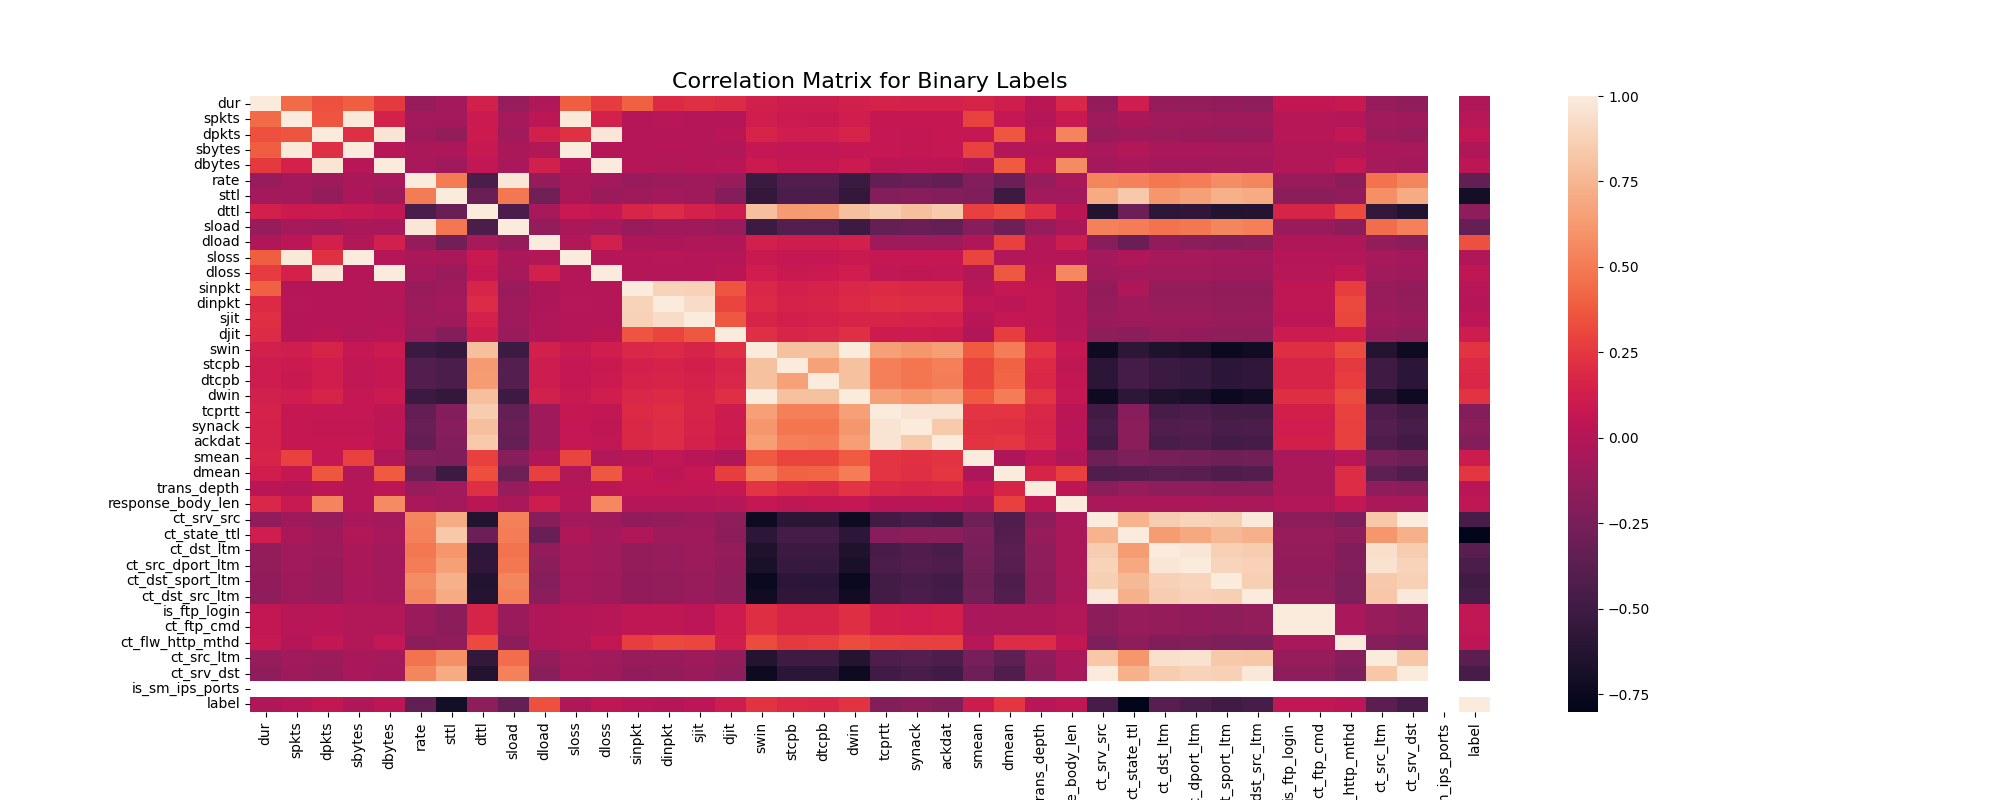
\includegraphics[width=5in,height=3in]{pic/correlation_matrix_bin.png}
\caption{Speaker recognition 3,person 1}
\end{figure}

\begin{figure} [hbtp]
\centering
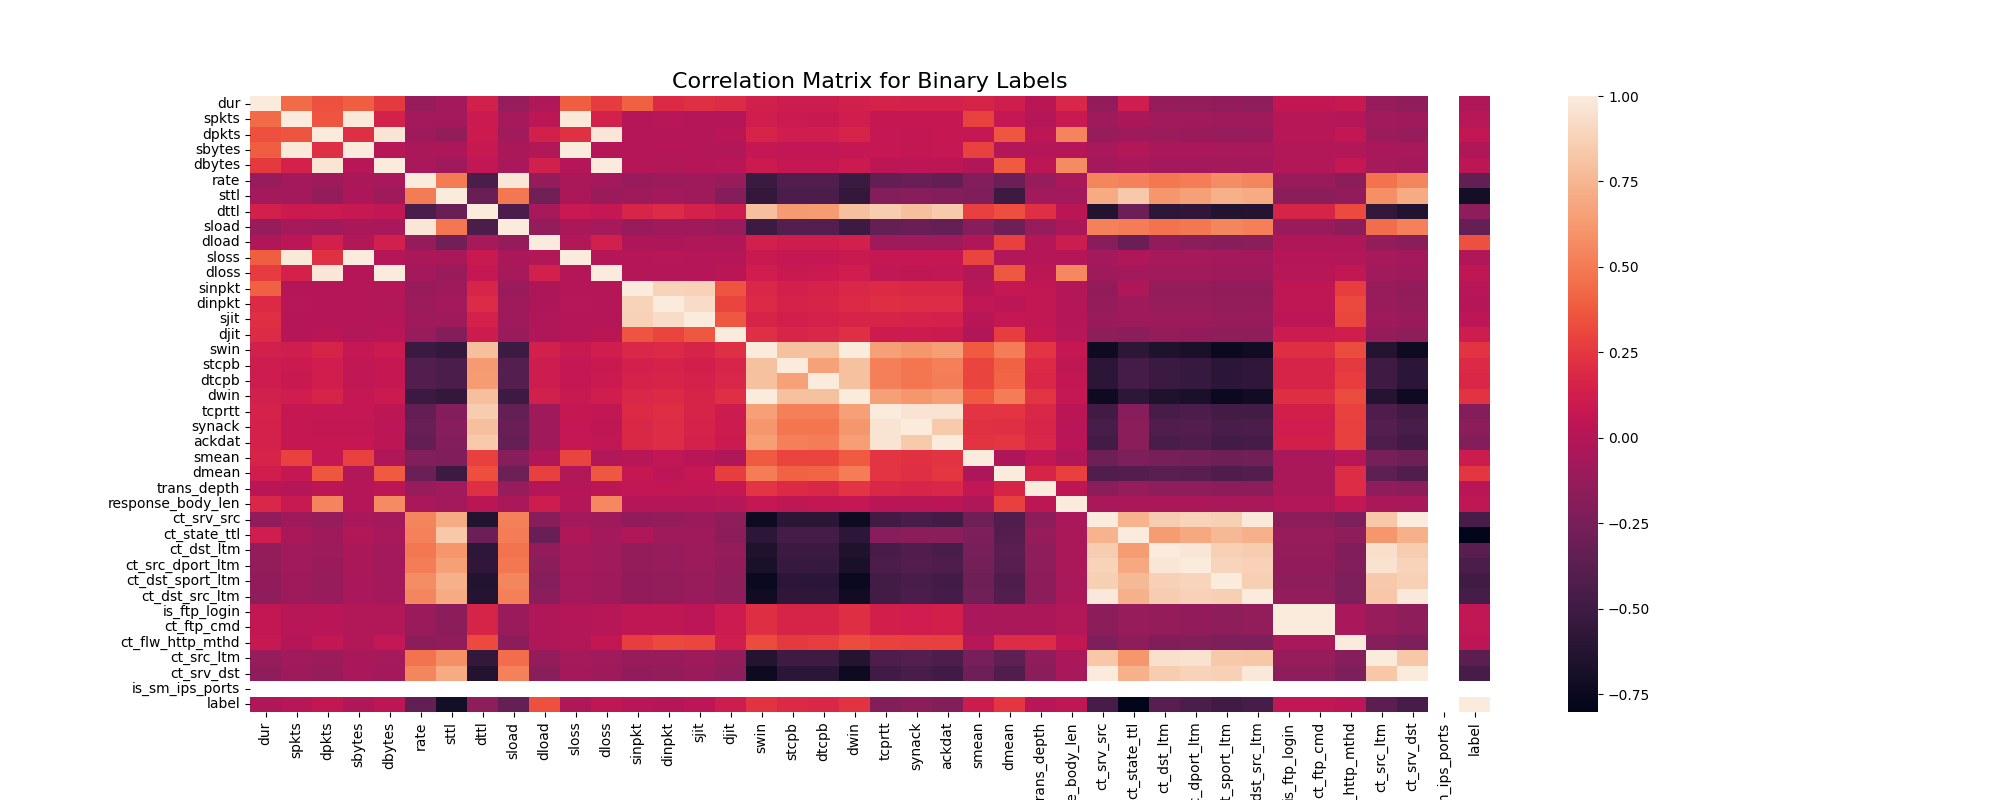
\includegraphics[width=5in,height=3in]{pic/correlation_matrix_bin.png}
\caption{Speaker recognition 3,person 2}
\end{figure}
\newpage
\par Above figures from 7.2 to 7.7 shows speaker recognition process using opencv and dlib.Speaker detection using cv2 and dlib involves utilizing dlib's pre-trained models along with cv2 functions to detect and locate human faces. By combining face detection with additional techniques such as audio analysis or lip movement tracking, speaker detection can be achieved in various applications like video conferencing or surveillance.

\chapter{Conclusion and Future work}
The Project will help in narrowing the imprecise communication problem in real-time data using 
speech separation and speaker identification technique by Deep Learning and Image Processing 
algorithms. This will impact the communication and security sectors in a greater extent. Overall, this 
project aims to develop an application or method that can help to separate the audio-visual speech and 
enhance it based on speaker identification.
\\
This project can be further developed as:
\item • By incorporating more real-world testing and gathering feedback from 
individual units.
\item • The system can be connected with communication devices or services to enable
the users to communicate with others with ease.
\\

This project has a great potential to make a positive impact on communication and security situations. Its continuous improvement will be important to make this impact 
even greater

\newpage
\pagestyle{plain}
\renewcommand{\bibname}{References}
\addcontentsline{toc}{chapter}{References}
\begin{thebibliography}{35}
\bibitem{ref1}
Hu, G., Yang, Y., Yi, D., Kittler, J., Christmas, W.J., Li, S., \& Hospedales, T.M. "When Face Recognition Meets with Deep Learning: An Evaluation of Convolutional Neural Networks for Face Recognition," 2015 IEEE International Conference on Computer Vision Workshop (ICCVW), pp. 384–392, Dec. 2015, doi: 10.1109/iccvw.2015.58.

\bibitem{ref2}
Parkhi, Omkar, Andrea Vedaldi, and Andrew Zisserman. "Deep face recognition." In BMVC 2015-Proceedings of the British Machine Vision Conference 2015. British Machine Vision Association, 2015.

\bibitem{ref3}
Levitin, Anany. "Introduction to design and analysis of algorithms", 2/E. Pearson Education India, 2008.

\bibitem{ref4}
Prabhu, "Understanding of Convolutional Neural Network (CNN) — Deep Learning", URL: https://medium.com/\@RaghavPrabhu/understanding-of-convolutional-neural-network-cnn-deep-learning-99760835f148. Accessed on 23/07/2023

\bibitem{ref5}
L. Blanger and A. R. Panisson, “A Face Recognition Library using Convolutional Neural Networks,” International Journal of Engineering Research and Science, vol. 3, no. 8, pp. 84–92, Aug. 2017, doi: 10.25125/engineering-journal-ijoer-aug-2017-25.
\bibitem{ref6}
R. Khedgaonkar, K. Singh, and M. Raghuwanshi, “Local plastic surgery-based face recognition using convolutional neural networks,” Demystifying Big Data, Machine Learning, and Deep Learning for Healthcare Analytics, pp. 215–246, 2021, doi: 10.1016/b978-0-12-821633-0.00001-5.
\bibitem{ref7}
P. J. Phillips, “A Cross Benchmark Assessment of a Deep Convolutional Neural Network for Face Recognition,” 2017 12th IEEE International Conference on Automatic Face \&; Gesture Recognition (FG 2017), pp. 705–710, May 2017, doi: 10.1109/fg.2017.89.
\bibitem{ref8}
Z. Huang, J. Zhang, and H. Shan, “When Age-Invariant Face Recognition Meets Face Age Synthesis: A Multi-Task Learning Framework,” 2021 IEEE/CVF Conference on Computer Vision and Pattern Recognition (CVPR), pp. 7278–7287, Jun. 2021, doi: 10.1109/cvpr46437.2021.00720.
\bibitem{ref9}
Z. Huang, J. Zhang, and H. Shan, “When Age-Invariant Face Recognition Meets Face Age Synthesis: A Multi-Task Learning Framework,” 2021 IEEE/CVF Conference on Computer Vision and Pattern Recognition (CVPR), pp. 7278–7287, Jun. 2021, doi: 10.1109/cvpr46437.2021.00720.
\end{thebibliography}


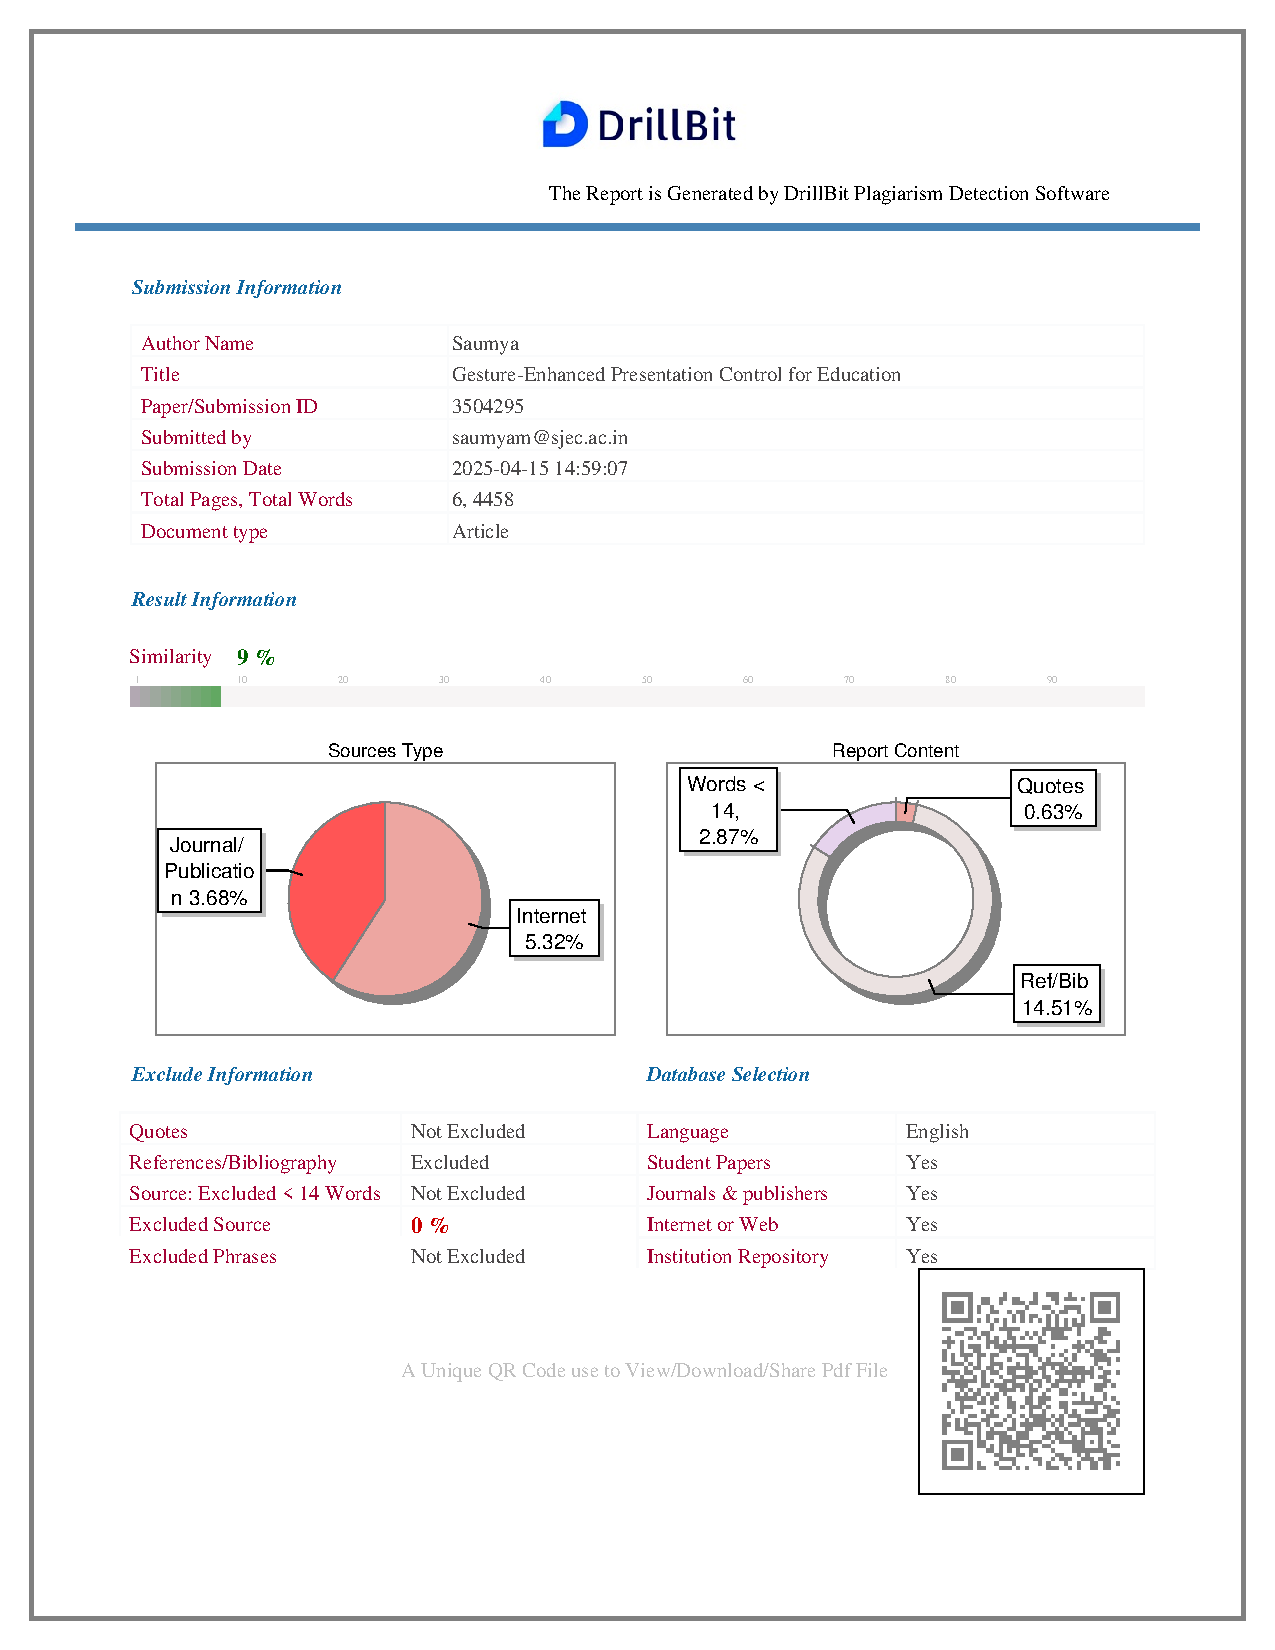
\includepdf[pages={1}]{DB_report_230-IEEE-Saumya.pdf}
% 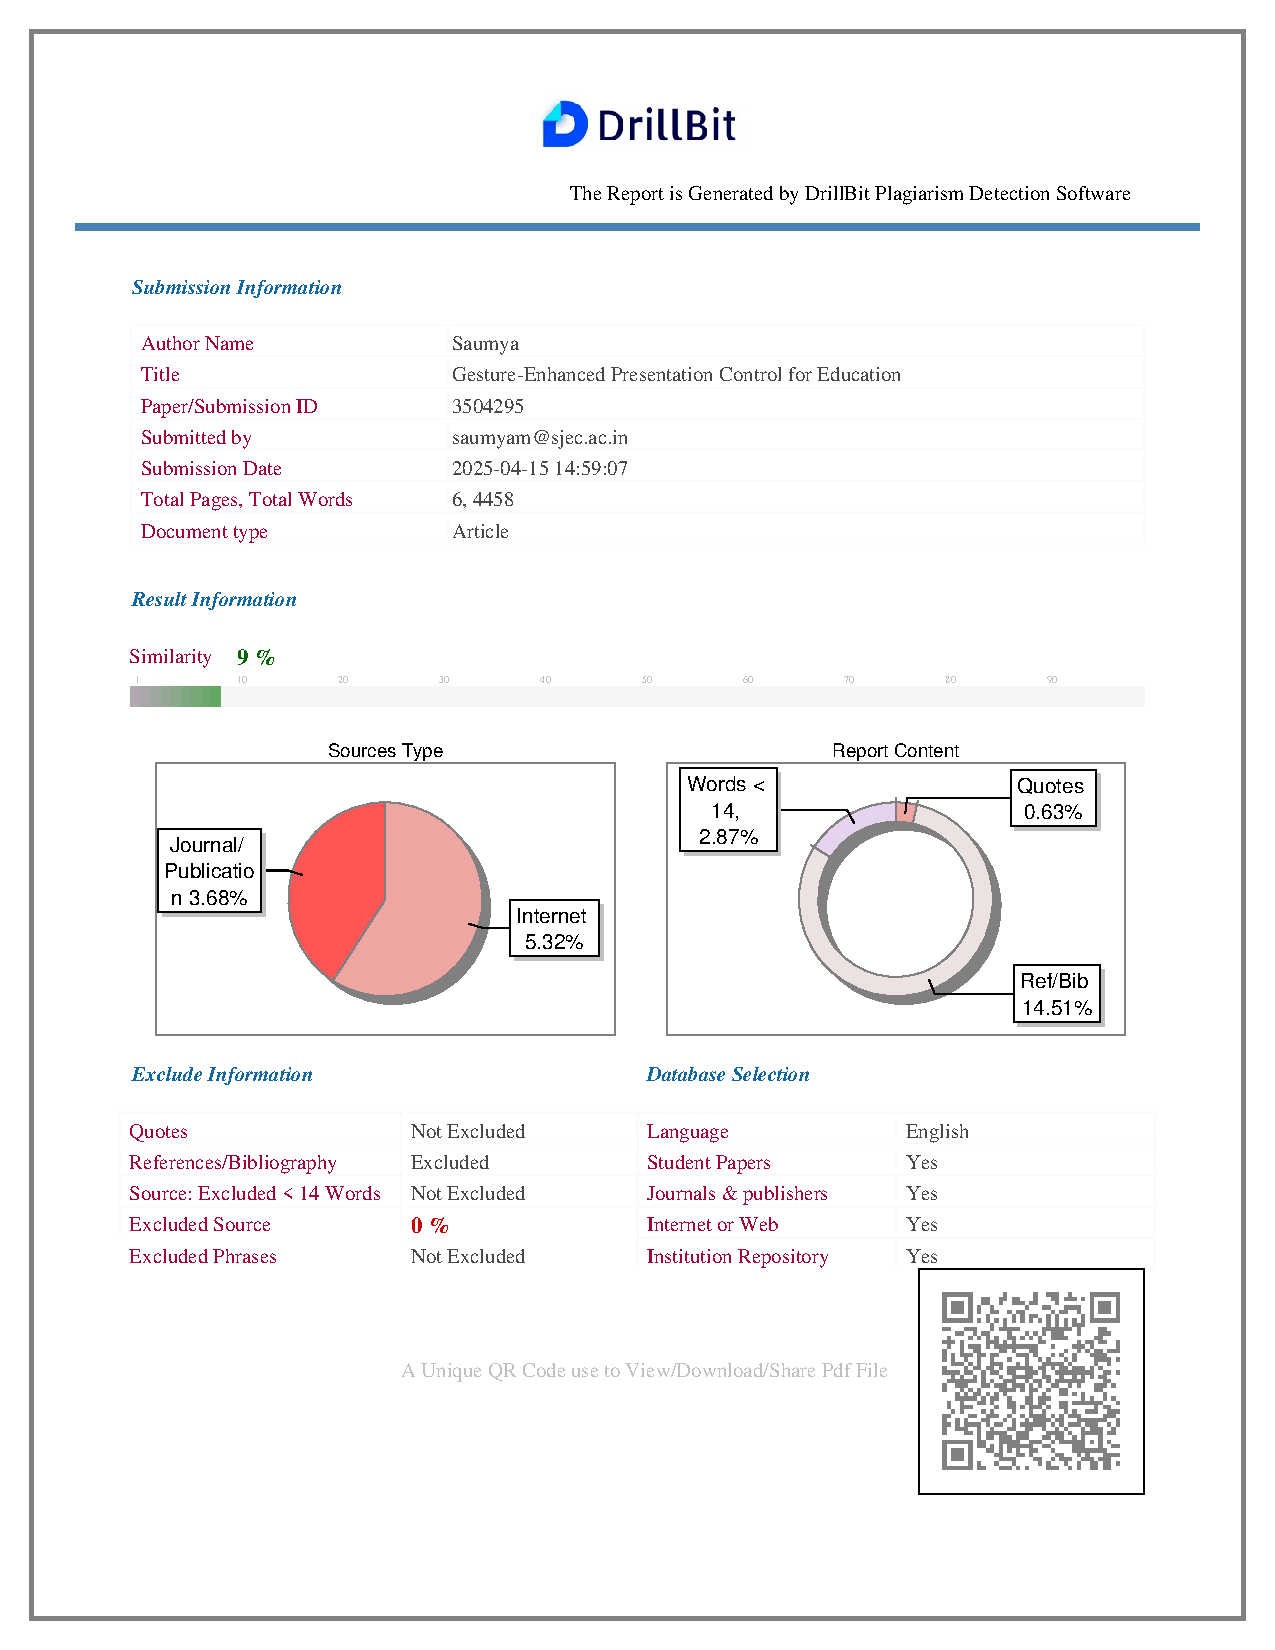
\includepdf[pages=-]{DB_Summary_report_230-IEEE-Saumya.pdf}
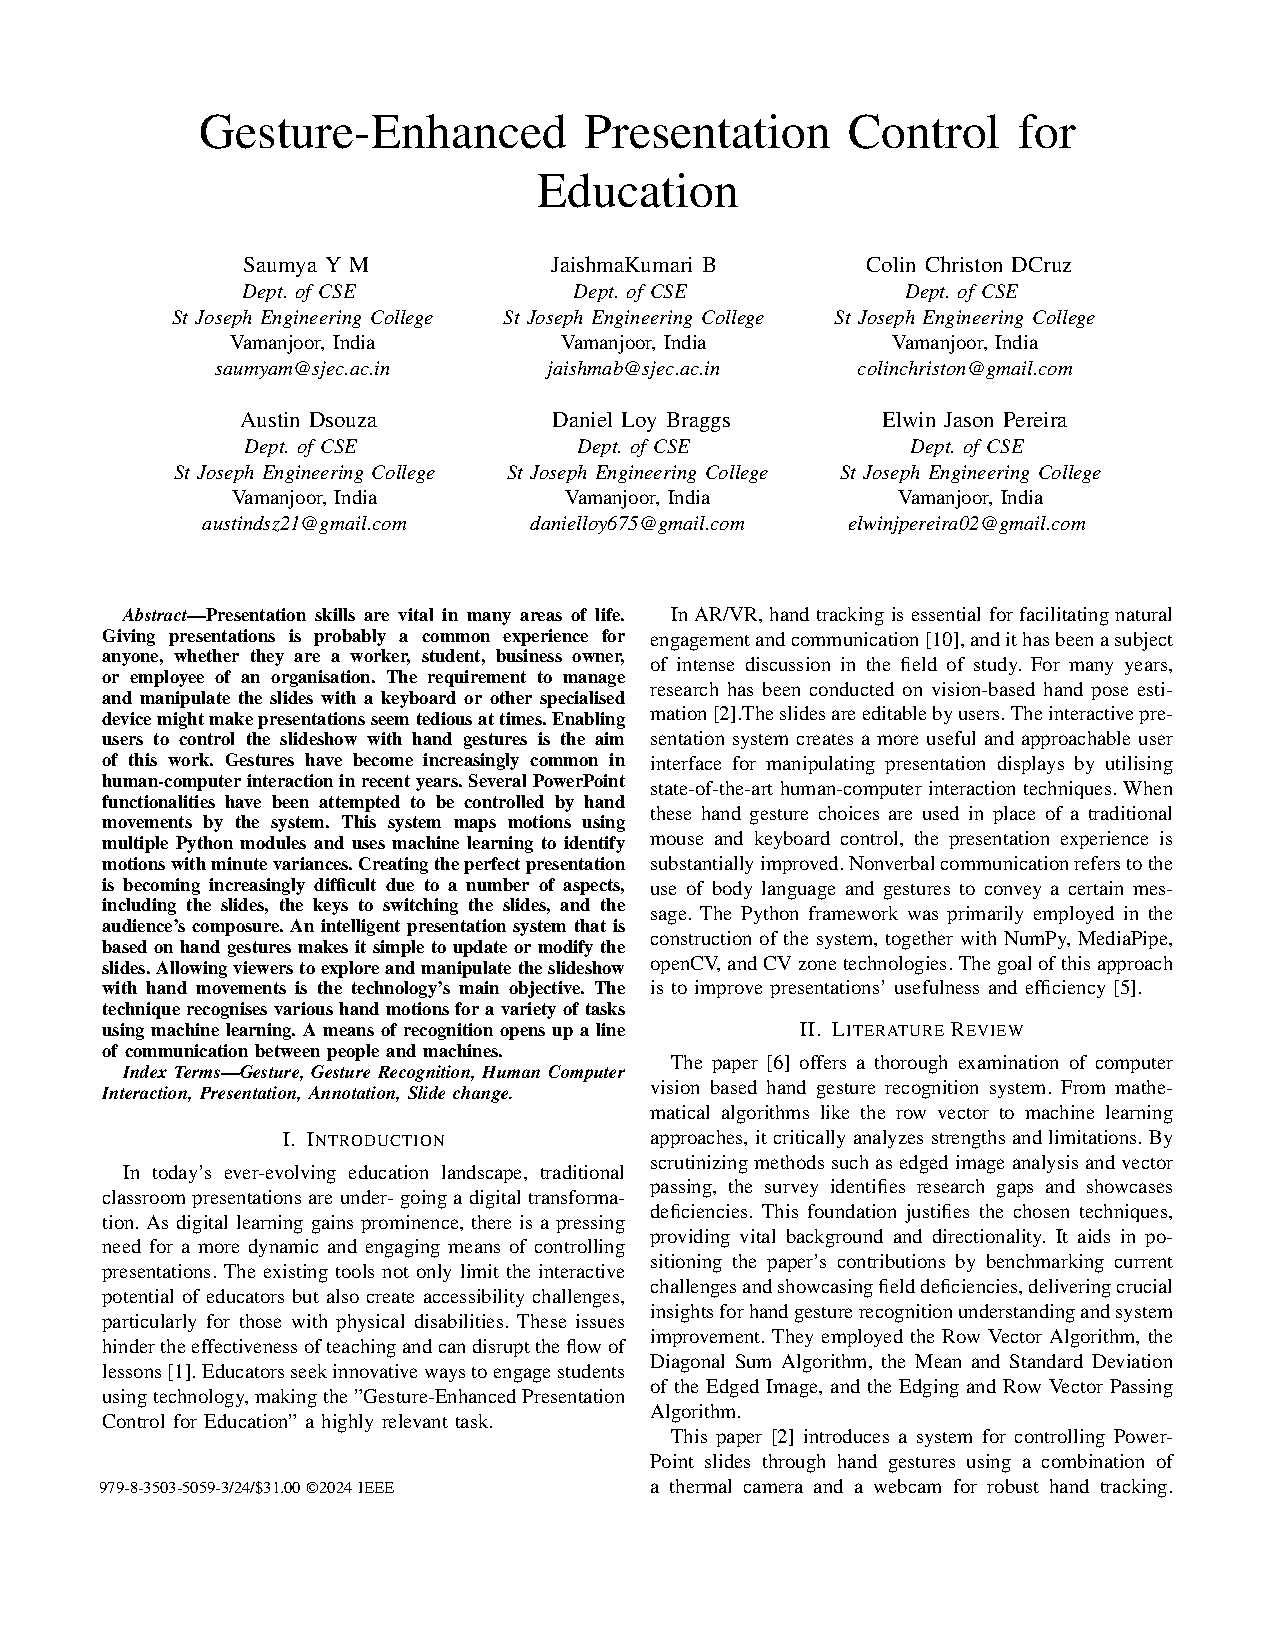
\includepdf[pages=-]{230-IEEE-Saumya.pdf}

\end{document}